
\section{Funcionamiento de Hardware}

\subsection{Microcontrolador ATmega328}
El ATmega es un microcontrolador de baja potencia CMOS de 8 bits. Mediante la ejecución de instrucciones potentes en un solo ciclo, el microcontrolador permite que el usuario optimice el consumo versus la velocidad de procesos. Este microcontrolador forma parte del Arduino UNO, el cual será la placa de hardware sobre la cual se desarrollará el control del vehículo en sus dos modalidades, seguidor de linea y control mediante bluetooh. 

La estructura del \textit{core} combina un conjunto robusto de instrucciones con 32 registros de trabajo. Estos 32 registros se encuentran directamente conectados a la Unidad
Lógica Aritmética (ALU), permitiendo el acceso independiente de dos registros ejecutados en un solo ciclo de reloj \cite{atmega}. 

\begin{figure}[H]
    \centering
    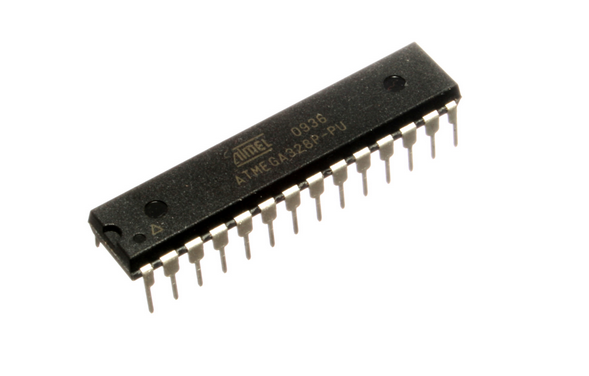
\includegraphics[width = 7 cm]{imagenes/micro.PNG}
    \caption{ATmega 328}
    \cite{atmega}
\end{figure}

\subsection{Sensor de obstáculo}
El sensor de obstáculo opera mediante una configuración emisor-receptor de luz infrarroja. Si la luz infrarroja choca contra un obstáculo, esta será reflejada y detectada por el fotodiodo. El rango de detección puede ser configurado mediante los dos controladores. Si no hay un obstáculo en frente la salida del sensor estará en alto, en el momento que se detecte un obstáculo la señal de salida se apagará.

El sensor permite activar o desactivar la detección de obstáculos mediante la manipulación del pin \textit{enable}. Por defecto, el sensor se encuentra en modo activo \cite{obstaculo}.

\begin{figure}[H]
    \centering
    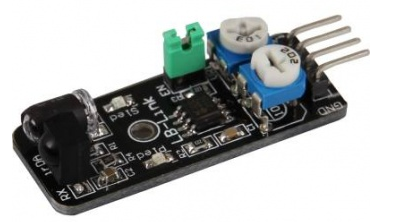
\includegraphics[width = 7 cm]{imagenes/obstacle.PNG}
    \caption{Sensor de obstáculo}
    \cite{obstaculo}
\end{figure}

\subsection{Sensor de traking}
Es un módulo tipo LEGO, listo para ser conectado al microcontrolador. Se basa en un sensor óptico reflexivo con salida de transistor, el cual se encarga de recibir las señales infrarrojas enviadas para detectar la intensidad de la señal. Con cierto rango de altura, los sensores de pista son ampliamente utilizados para vehículos inteligentes o impresoras para detección de líneas en blanco y negro \cite{track}.

\begin{figure}[H]
    \centering
    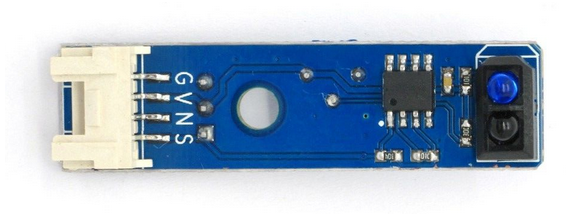
\includegraphics[width = 7 cm]{imagenes/tracking.png}
    \caption{Sensor de pista}
    \cite{track}
\end{figure}


\subsection{Motores DC 200 RPM a escala}
Compuesto por un par de motores DC a escala, son usualmente recomendados como una opción barata y sencilla para poner ruedas en movimiento. Requieren una tensión de 4.5V y una corriente sin carga de 190 mA además posee una caja reductora 48:1 y una velocidad de giro de 200 RPM sin carga \cite{motor_dc}.

\begin{figure}[H]
    \centering
    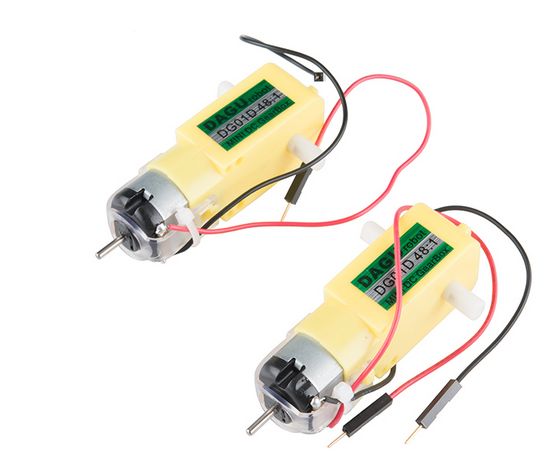
\includegraphics[width = 7 cm]{imagenes/gearmotor.PNG}
    \caption{Hobby Gearmotor - 200 RPM}
    \cite{motor_dc}
\end{figure}

\subsection{Módulo de control de motores DC 800 mA}

El módulo de control L9110S 2-Canales es una tarjeta compacta que puede ser utilizada para controlar robots pequeños. Este módulo posee dos controladores independientes capaces de entregar hasta 800 mA en corriente continua. Pueden operar entre 2.5V y 12V lo cual permite que sean usados mediante microcontroladores.

Mediande control PWM ---\textit{Pulse Width Modulation}--- es posible controlar la velocidad del motor y una salida digital es usada para indicar la dirección \cite{driver}.

\begin{figure}[H]
    \centering
    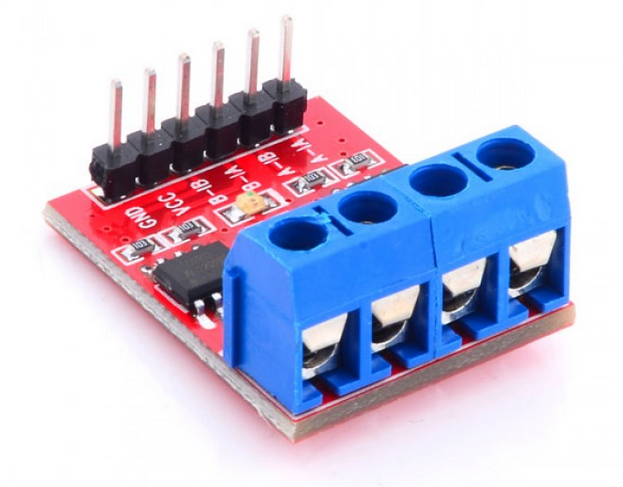
\includegraphics[width = 7 cm]{imagenes/driver.PNG}
    \caption{L9110S Drive Dual Motor DC 800mA}
    \cite{driver}
\end{figure}


\subsection{Servomotor}
El servo es un tipo de motor que funciona paso-a-paso, es decir, su giro se determina en ángulos y no en RPM. Pequeño, liviano y con una alta potencia de salida; este tipo de servomotor es capaz de rotar hasta 180 grados \cite{servo}.

\begin{figure}[H]
    \centering
    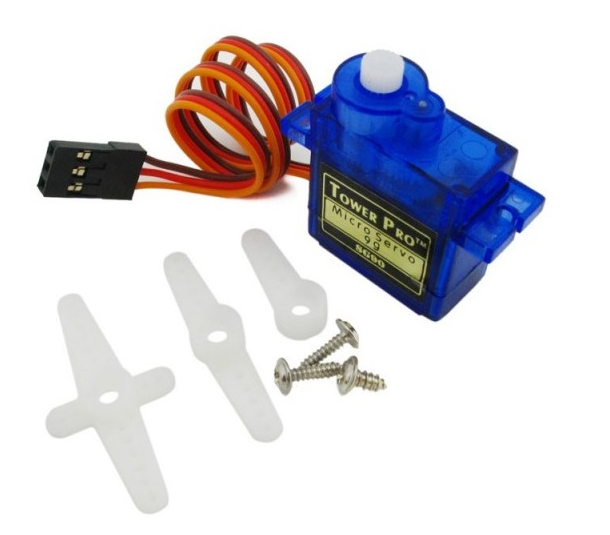
\includegraphics[width = 7 cm]{imagenes/servo.PNG}
    \caption{Servomotor SG90}
    \cite{servo}
\end{figure}

\subsection{Piezo Speaker}
Es un pequeño parlante redondo de 12mm el cual opera en todo el rango audible. Pueden ser utilizados para crear interfaces simples musicales. Requiere de una tensión entre los 3.5V y 5V con una corriente media de 35 mA además de una onda cuadrada para su correcto funcionamiento.

\begin{figure}[H]
    \centering
    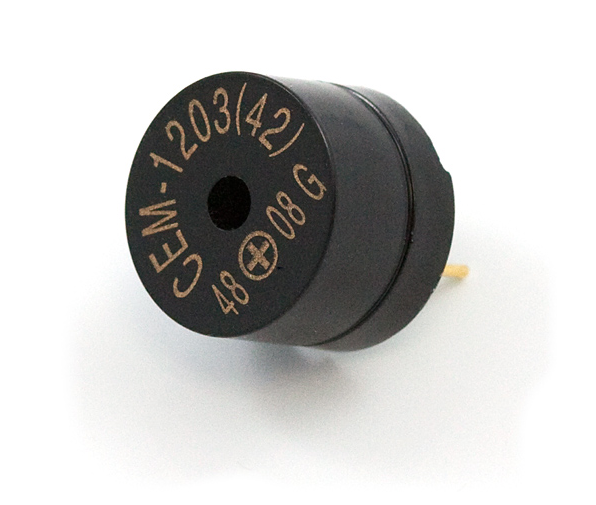
\includegraphics[width = 7 cm]{imagenes/speaker.PNG}
    \caption{Magnetic buzzer}
    \cite{speaker}
\end{figure}

Leer más: \url{https://www.microjpm.com/products/buzzer-timbre-tono-de-alarma-1-5v-3v-6v-12v/}

\subsection{Módulo bluetooth HC-05}
El módulo bluetooth HC-05 se utiliza en este proyecto para poder enviar datos desde un programa en C al arduino, la comunicación se realiza a través del puerto serial, mediante el cual se transmiten los datos. Dichos datos son interpretados por el arduino para llevar a cabo las funciones que el vehículo realiza. 
\begin{figure}[H]
    \centering
    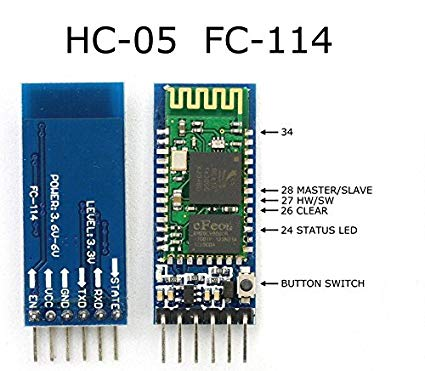
\includegraphics[width= 7 cm]{./imagenes/hc-05.jpg}
    \caption{Módulo bluetooth}
   
\end{figure}


\subsection{Esquemático de conexiones de vehículo}

\begin{figure}[H]
    \centering
    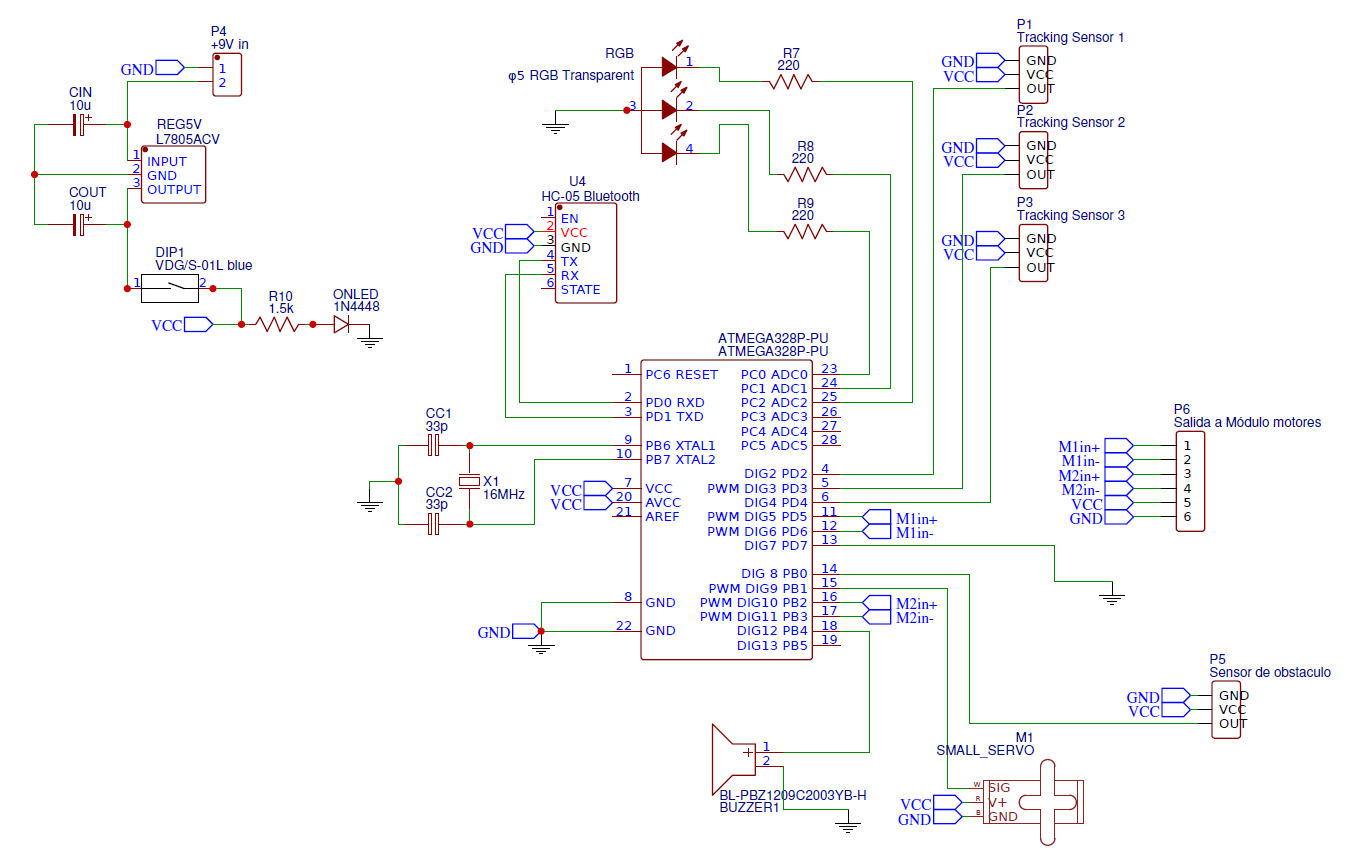
\includegraphics[width = 18 cm]{imagenes/schem_vehiculo.PNG}
    \caption{Esquemático del Vehículo Seguidor de Línea}
\end{figure}
